\documentclass[letterpaper,twocolumn,fleqn]{article} 

\pagestyle{empty}                % no page numbers is default

\usepackage{amsfonts}
\usepackage{amssymb}
\usepackage[cmex10]{amsmath}
\usepackage{booktabs}
\usepackage{caption}
\usepackage{enumitem}
\usepackage{graphicx}
\usepackage{fancyvrb}
\usepackage{framed}
\usepackage{ifthen}
\usepackage{cite}
\usepackage{tabulary}
\usepackage{url}
\usepackage{xspace}
\usepackage{wrapfig}
\usepackage[pdfborder={0 0 0}]{hyperref}
\usepackage{verbatim}

\usepackage{ist} % Style for IST in package instead of document class.

\usepackage{color}
\definecolor{yellow}{rgb}{1,1,0}
\definecolor{black}{rgb}{0,0,0}
\definecolor{ltcyan}{rgb}{.75,1,1}
\definecolor{red}{rgb}{1,0,0}
\definecolor{gray}{rgb}{.6,.6,.6}
\definecolor{darkred}{rgb}{0.5,0,0}
\definecolor{darkgreen}{rgb}{0,0.5,0}

% Cite commands I use to abstract away the different ways to reference an
% entry in the bibliography (superscripts, numbers, dates, or author
% abbreviations).  \scite is a short cite that is used immediately after
% when the authors are mentioned.  \lcite is a full citation that is used
% anywhere.  Both should be used right next to the text being cited without
% any spacing. \hcite is a citation that I am hiding, perhaps because I am
% nearing the maximum number of citations for a journal.
\newcommand*{\lcite}[1]{~\cite{#1}}
\newcommand*{\scite}[1]{~\cite{#1}}
\newcommand*{\hcite}[1]{}

\newcommand{\etal}{et al.\xspace}

\newcommand*{\keyterm}[1]{\emph{#1}}

\newcommand{\fix}[1]{{\color{red}\textsc{[#1]}}}
%\newcommand{\fix}[1]{}

% Avoid putting figures on their own page.
\renewcommand{\textfraction}{0.05}
\renewcommand{\topfraction}{0.95}
\renewcommand{\bottomfraction}{0.95}

% Make sure this is big enough so that only big figures end up on their own
% page but small enough so that if a figure does have to be on its own
% page, it won't push everything to the bottom because it's not big enough
% to have its own page.
\renewcommand{\floatpagefraction}{.75}


\title{Why We Use Bad Color Maps and What You Can Do About It}

\author{Kenneth Moreland; Sandia National Laboratories; Albuquerque, New
  Mexico, USA}

\date{} % date has an empty field.

% correct for bad hyphenation here
\hyphenation{Para-View}

\begin{document} 

\maketitle 

\thispagestyle{empty} % prevents the first page to be numbered

\begin{abstract}
\noindent
We know the rainbow color map is terrible and emphatically reviled by the
visualization community, yet its use continues to persist. Why do we
continue to use a this perceptual encoding with so many known flaws?
Instead of focusing on why we should not use rainbow colors, this position
statement explores the rational for why we do pick these colors despite
their flaws. Often the decision is influenced by a lack of knowledge, but
even experts that know better sometimes choose poorly. A larger issue is
the expedience that we have inadvertently made the rainbow color map
become. Knowing why the rainbow color map is used will help us move away
from it. Education is good, but clearly not sufficient. We gain traction by
making sensible color alternatives the more convenient alternative. It is
not feasible to force a color map on users. Our goal is to supplant the
rainbow color map as a common standard, and we will find that even those
wedded to it will migrate away.
\end{abstract}


\section{Introduction}

\noindent
A pervasive technique in scientific visualization called pseudocoloring is
to apply colors to an object that vary based on some numerical variable.
Pseudocoloring requires defining a function or map from numerical values to
colors. A color map is typically defined by selecting a continuum of colors
that map linearly to a range of numeric values.
Figure~\ref{fig:ColorMapExample} shows a simple example of a color map
where numeric values between -1 and 0 map to blue colors of varying
brightness and numeric values between 0 and 1 map to red colors.

\begin{figure}[htb]
  \centering
  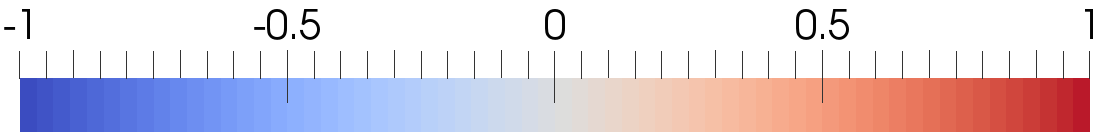
\includegraphics[width=.9\linewidth]{images/ColorMapExample}
  \caption{A simple example of a color map.}
  \label{fig:ColorMapExample}
\end{figure}

The efficacy of a pseudocolor visualization is contingent on the ability of
a human observer to translate the colors back into the numeric values they
represent. The choice of colors used in a pseudocolor map can have a major
impact on this inverse translation. Consequently, much research has focused
on the perception of color and its impact of the visual display of
data\fix{cite stone, brewer, ware, reigens, rogowitz}.


\section{Why We Use Bad Colors}


\section{How We Can Promote Good Color Use}


\section{Practical Considerations}

Managing the unknown.


\section{Acknowledgments} 

% To start a new column (but not a new page) and help balance the last-page
% column length use \vfill\pagebreak.

\small
\bibliographystyle{plain}
%% \bibliography{BadColorMaps}

\begin{biography}
\noindent
Dr. Kenneth Moreland is a principal member of technical staff at Sandia
National Laboratories. He received the BS degrees in computer science and
electrical engineering from New Mexico Tech in 1997. He received MS and
Ph.D. degrees in computer science from the University of New Mexico in
2000, and 2004, respectively. Dr. Moreland specializes in large-scale
visualization and plays an active role in several HPC products including
ParaView, VTK, IceT, Dax, and VTK-m.
\end{biography}

\end{document} 
